\documentclass[12pt]{article}

\setlength{\oddsidemargin}{0in}  %left margin position, reference is one inch
\setlength{\textwidth}{6.5in}    %width of text=8.5-1in-1in for margin
\setlength{\topmargin}{-0.5in}    %reference is at 1.5in, -.5in gives a start of about 1in from top
\setlength{\textheight}{9in}     %length of text=11in-1in-1in (top and bot. marg.) 

\usepackage[square,super]{natbib}
\usepackage{graphicx}
\usepackage[dvipsnames]{xcolor}

\usepackage{multirow}
\usepackage{subcaption}
\usepackage{setspace}
\usepackage{xfrac}
\usepackage{hyperref}
\usepackage{upgreek}
\usepackage{lscape}
\usepackage{mhchem}
\usepackage{longtable}
\usepackage{rotating}
%\usepackage{fancyhdr}

\hypersetup{colorlinks=true,citecolor=black,linkcolor=blue, urlcolor=blue}

\usepackage{tikz}
%\usepackage[numbers,super,comma,sort&compress]{natbib}
%\usepackage[scaled=0.95]{helvet}
%\renewcommand{\familydefault}{\sfdefault}
\usepackage{amssymb}
\usepackage{amsmath}
\usepackage{placeins}
\usepackage[final]{pdfpages}

\usepackage{listings} %provides code listings
\definecolor{codegreen}{rgb}{0,0.6,0}
\definecolor{codegray}{rgb}{0.5,0.5,0.5}
\definecolor{codepurple}{rgb}{0.58,0,0.82}
\definecolor{backcolour}{rgb}{0.95,0.95,0.92}
\lstdefinestyle{mystyle}{
    backgroundcolor=\color{backcolour},   
    commentstyle=\color{codegreen},
    keywordstyle=\color{magenta},
    numberstyle=\tiny\color{codegray},
    stringstyle=\color{codepurple},
    basicstyle=\ttfamily\scriptsize,
    breakatwhitespace=false,         
    breaklines=true,                 
    captionpos=b,                    
    keepspaces=true,                 
    numbers=left,                    
    numbersep=5pt,                  
    showspaces=false,                
    showstringspaces=false,
    showtabs=false,                  
    tabsize=2
}
\lstset{style=mystyle}


\newcommand*{\citen}[1]{%
  \begingroup
    \romannumeral-`\x % remove space at the beginning of \setcitestyle
    \setcitestyle{numbers}%
    \cite{#1}%
  \endgroup   
}

\setlength{\parskip}{0pt}


\definecolor{C0}{HTML}{1F77B4}
\definecolor{C1}{HTML}{FF7F0E}
\definecolor{C2}{HTML}{2CA02C}
\definecolor{C3}{HTML}{D62728}
\definecolor{C4}{HTML}{9467BD}
\definecolor{C5}{HTML}{8C564B}
\definecolor{C6}{HTML}{E377C2}
\definecolor{C7}{HTML}{7F7F7F}
\definecolor{C8}{HTML}{BCBD22}
\definecolor{C9}{HTML}{17BECF}


\newcommand{\tcn}[1]{{#1}}
\newcommand{\tcr}[1]{{#1}}
%\newcommand{\tcr}[1]{\textcolor{red}{#1}}

\newcommand{\beginsupplement}{%
        \setcounter{table}{0}
        \renewcommand{\thetable}{S\arabic{table}}%
        \setcounter{figure}{0}
        \renewcommand{\thefigure}{S\arabic{figure}}%
        \renewcommand{\thepage}{S\arabic{page}}%
     }

%\pagestyle{fancy}
%\fancyhf{}
%\cfoot{S\thepage}

\begin{document}

\title{Towards automation of operando experiments: A case study in contactless conductivity measurements}

\date{Supplementary Material}

\author{P.~Kraus,\thanks{E-Mail: peter.kraus@curtin.edu.au}\hspace{7pt}E.~H.~Wolf,
        C.~Prinz, G.~Bellini, A.~Trunschke, and R.~Schl\"{o}gl}

\maketitle


%%%END OF FOOTNOTES%%%

%%%MAIN TEXT%%%%

\beginsupplement

\section*{Table of contents}
\begin{enumerate}
	\item Excerpt from an \emph{instrument log} file. \hfill p.~S2
    \item Excerpt from a \emph{VNA log} file. \hfill p.~S3
	\item Summary of the MCPT data for samples activated in \ce{C3}-oxidation, studied with the \emph{Handbook} protocol. The full archive, including \emph{datagrams}, \emph{schema} files, \emph{parameter files}, and all raw data, is available at DOI:~\href{https://doi.org/10.5281/zenodo.5008960}{10.5281/zenodo.5008960}  \hfill p.~S4
    \item Summary of the MCPT data for other samples studied with the \emph{Handbook} protocol. The full archive, including \emph{datagrams}, \emph{schema} files, \emph{parameter files}, and all raw data, is available at DOI:~\href{https://doi.org/10.5281/zenodo.5010992}{10.5281/zenodo.5010992}  \hfill p.~S4
    \item Summary of the MCPT data for samples studied with the perovskite protocol. The full archive, including \emph{datagrams}, \emph{schema} files, \emph{parameter files}, and all raw data, is available at DOI:~\href{https://doi.org/10.5281/zenodo.4980210}{10.5281/zenodo.4980210} \hfill p.~S5
    \item Piping and instrumentation diagram of the MCPT instrument \hfill p.~S6
	\item Technical diagram of the MCPT dewar \hfill p.~S7
	\item Technical diagram of a MCPT reactor \hfill p.~S8
	\item Illustration of the MCPT dewar/reactor assembly \hfill p.~S9
\end{enumerate}

Additional supplemental files and archives in computer-readable form are available on Zenodo, see DOI: \href{http://dx.doi.org/10.5281/zenodo.4783007}{10.5281/zenodo.4783007}. An executable version of this archive is available on \href{https://mybinder.org/v2/zenodo/10.5281/zenodo.4783007/?filepath=index.ipynb}{Binder}.

\clearpage
\begin{landscape}
\begin{figure}[tbh]
\begin{lstlisting}[escapechar=£,
    linewidth=24cm]
£\colorbox{green!35}{timestamp; elapsed; T\_f; T\_fs; T\_fo; T\_c; T\_cs; T\_co; N2; O2; alkane; CO/CO2; sat.; press.; flow low; flow high; cav. flush; heater flow; T\_cal}£
; ; C; C; \%; C; C; \%; ml/min; ml/min; ml/min; ml/min; ml/min; mbar; ml/min; ml/min; ml/min; l/min; C
2019-08-29-16-36-37; 0h 1m 0s;22.9;21.6;0.0;18;18;-12;28.12;1.48;0.00;0.00;0.00;1300.6;1.210;0.00;15;8;20.6
2019-08-29-16-37-37; 0h 2m 0s;22.9;23.6;1.3;18;18;-6;28.12;1.48;0.00;0.00;0.00;1299.7;1.210;0.00;15;8;21.0
2019-08-29-16-38-38; 0h 3m 1s;23.1;25.6;9.3;18;18;-11;28.12;1.48;0.00;0.00;0.00;1299.4;1.209;0.00;15;8;20.5
2019-08-29-16-39-39; 0h 4m 2s;26.0;27.7;11.8;18;18;-12;28.12;1.48;0.00;0.00;0.00;1300.3;1.211;0.00;15;8;21.0
2019-08-29-16-40-39; 0h 5m 2s;29.0;29.7;12.1;18;18;-18;28.13;1.48;0.00;0.00;0.00;1300.0;1.210;0.00;15;8;20.3
2019-08-29-16-41-40; 0h 6m 3s;31.1;31.7;13.0;18;18;-8;28.11;1.48;0.00;0.00;0.00;1299.7;1.210;0.00;15;8;20.1
2019-08-29-16-42-40; 0h 7m 3s;33.1;33.7;13.9;18;18;-10;28.12;1.48;0.00;0.00;0.00;1300.0;1.211;0.00;15;8;20.3
2019-08-29-16-43-40; 0h 8m 4s;35.1;35.7;14.7;18;18;-12;28.12;1.48;0.00;0.00;0.00;1299.7;1.210;0.00;15;8;20.3
2019-08-29-16-44-41; 0h 9m 4s;37.2;37.7;15.4;18;18;-2;28.12;1.48;0.00;0.00;0.00;1299.4;1.212;0.00;15;8;20.9
2019-08-29-16-45-41; 0h10m 5s;39.2;39.7;16.1;18;18;-17;28.12;1.48;0.00;0.00;0.00;1299.7;1.210;0.00;15;8;21.9
                    [...]
2019-08-29-18-46-08; 2h10m32s;252.0;252.0;48.6;18;18;-7;28.11;1.48;0.00;0.00;0.00;1300.0;1.211;0.00;15;8;20.2
2019-08-29-18-47-09; 2h11m32s;252.0;252.0;48.7;18;18;-20;28.12;1.48;0.00;0.00;0.00;1300.6;1.211;0.00;15;8;20.2
2019-08-29-18-48-09; 2h12m32s;252.0;252.0;48.8;18;18;-22;28.12;1.48;0.00;0.00;0.00;1300.6;1.211;0.00;15;8;20.2
2019-08-29-18-49-10; 2h13m33s;252.0;252.0;48.5;18;18;-17;28.12;1.48;0.00;0.00;0.00;1300.0;1.212;0.00;15;8;20.7
2019-08-29-18-50-11; 2h14m34s;252.0;252.0;48.8;18;18;-19;28.12;1.48;0.00;0.00;0.00;1300.0;1.211;0.00;15;8;20.6
2019-08-29-18-51-11; 2h15m34s;252.3;252.8;49.7;18;18;-18;28.12;3.32;7.32;0.00;0.00;1300.0;0.653;0.95;15;8;20.6
2019-08-29-18-52-12; 2h16m36s;254.4;254.8;49.3;18;18;-16;28.12;3.32;7.33;0.00;0.00;1300.6;0.656;0.98;15;8;20.8
2019-08-29-18-53-13; 2h17m37s;256.4;256.8;49.8;18;18;-20;28.12;3.32;7.34;0.00;0.00;1300.6;0.656;1.00;15;8;20.1
2019-08-29-18-54-14; 2h18m37s;258.5;258.9;49.9;18;18;-15;28.12;3.32;7.35;0.00;0.00;1300.0;0.656;0.99;15;8;19.9
2019-08-29-18-55-16; 2h19m39s;260.5;260.9;50.3;18;18;-18;28.12;3.32;7.33;0.00;0.00;1300.6;0.656;1.00;15;8;19.8
                    [...]
2019-08-31-20-31-59;51h56m22s;423.0;423.0;68.3;19;18;-40;28.12;3.32;7.36;0.00;0.00;1299.7;0.656;0.00;15;8;21.5
2019-08-31-20-33-00;51h57m23s;423.0;423.0;68.4;19;18;-30;28.12;3.32;7.34;0.00;0.00;1300.0;0.657;0.00;15;8;21.5
2019-08-31-20-34-01;51h58m24s;423.0;423.0;68.2;19;18;-32;28.12;3.32;7.34;0.00;0.00;1300.3;0.656;0.00;15;8;21.6
2019-08-31-20-35-01;51h59m25s;423.0;423.0;68.2;19;18;-31;28.12;3.32;7.34;0.00;0.00;1299.4;0.656;0.00;15;8;20.9
2019-08-31-20-36-02;52h 0m25s;411.1;20.0;0.0;19;18;-29;28.13;1.65;0.00;0.00;0.00;1294.4;1.260;24.43;15;8;21.2
2019-08-31-20-37-02;52h 1m25s;285.8;20.0;0.0;19;18;-32;28.12;1.48;0.00;0.00;0.00;1300.0;1.211;0.99;15;8;21.1
2019-08-31-20-38-03;52h 2m26s;172.5;20.0;0.0;18;18;-12;28.12;1.48;0.00;0.00;0.00;1299.7;1.210;0.99;15;8;21.3
2019-08-31-20-39-03;52h 3m26s;105.2;20.0;9.9;18;18;-20;28.12;1.48;0.00;0.00;0.00;1299.7;1.211;0.99;15;8;21.6
2019-08-31-20-40-05;52h 4m28s;69.7;20.0;0.0;18;18;-17;28.12;1.48;0.00;0.00;0.00;1299.7;1.211;1.00;15;8;21.8
2019-08-31-20-41-06;52h 5m29s;51.3;20.0;0.0;18;18;-17;28.12;1.48;0.00;0.00;0.00;1299.7;1.211;1.00;15;8;20.9
\end{lstlisting}
\centering
\caption{Excerpt from an \emph{instrument log} file, showing an example of start-up with a ramp reaching 252°C at 2°C/min (3-12), switch of feed from oxidative to reaction (14-23) and cooldown procedure (25-34). The header (highlighted in green) lists the columns, which correspond to the timestamp, elapsed run time, inlet temperature, inlet temperature setpoint, heater duty cycle, cavity temperature, cavity temperature setpoint, Peltier duty cycle, \ce{N2} flow, \ce{O2} flow, alkane flow, \ce{CO}/\ce{CO2} flow, saturator flow, inlet pressure, inlet flow (meter no.~1), inlet flow (meter no.~2), cavity flush, heater medium flow, temperature of the calibration thermocouple. \label{fig:instlog}}
\end{figure}
\end{landscape}
\clearpage

\begin{figure}[tbh]
\begin{lstlisting}[escapechar=£]
£\colorbox{green!35}{BW = 10000;AVG = 10}£
+7.100000E+9	-2.280313E-2	+9.412804E-1
+7.100015E+9	-2.241943E-2	+9.409110E-1
+7.100030E+9	-2.244101E-2	+9.406135E-1
+7.100045E+9	-2.181034E-2	+9.407906E-1
+7.100060E+9	-2.154459E-2	+9.396642E-1
+7.100075E+9	-2.166180E-2	+9.403051E-1
+7.100090E+9	-2.122021E-2	+9.408551E-1
+7.100105E+9	-2.164769E-2	+9.408164E-1
+7.100120E+9	-2.139573E-2	+9.404883E-1
+7.100135E+9	-2.145294E-2	+9.407361E-1
   [...]
+7.399865E+9	-2.219277E-2	-9.154096E-1
+7.399880E+9	-2.249969E-2	-9.151102E-1
+7.399895E+9	-2.282277E-2	-9.154791E-1
+7.399910E+9	-2.304419E-2	-9.154005E-1
+7.399925E+9	-2.431337E-2	-9.159150E-1
+7.399940E+9	-2.515590E-2	-9.163996E-1
+7.399955E+9	-2.466450E-2	-9.154912E-1
+7.399970E+9	-2.516757E-2	-9.149708E-1
+7.399985E+9	-2.563848E-2	-9.151121E-1
+7.400000E+9	-2.602740E-2	-9.156989E-1
\end{lstlisting}
\centering
\caption{Excerpt from a \emph{VNA log} file. Only the header (highlighted in green) and the first and last 10 lines shown. The header lists the filter bandwidth (10000~Hz) and number of shots averaged (10). The columns correspond to the frequency $f$ and the real and complex parts of the reflection coefficient $\Upgamma(f)$. \label{fig:vnalog}}
\end{figure}

\clearpage
\begin{landscape}
\begin{table}[p]
\caption{Results of the operando MCPT investigations of transition metal oxide samples, activated in \ce{C3}-oxidation, using the \emph{Handbook} protocol. Columns include the name and nominal atomic composition, sample ID, reference conductivity at 300$^\circ$C, activation energy of conductivity, changes in conductivity as a function of inlet stoichiometry and residence time, activation energy of mass-normalized conversion, the ideality of conversion with residence time, and interpolated selectivities to CO$_x$ and \ce{C3H6} at 5\% conversion (dashes correspond to cases where $X$ is well below or above 5\%). \label{tab:hbook}}
\small
\begin{tabular}{l|l|r|r|r|r|r|r|r|r}
Sample name & Sample ID & $\sigma_r$& $E_A(\sigma)$ & $\Delta \sigma (\phi)$ & $\Delta \sigma (\tau)$ & $E_A(X/m)$ & $\Delta X(\tau)/X$ & $S_{\mathrm{CO}_x}(5\%)$ & $S_{\mathrm{C}_3\mathrm{H}_6}(5\%)$\\
 & & [S/m] & [kJ/mol] & [S/m] & [S/ms] & [kJ/mol] & [\%] & [\%] & [\%]\\
\hline
"VPP"-C$_3$ & 32082 & $0.005(4)$ & $20(1)$ & $0.0067(7)$ & $-0.00018(6)$ & $16(31)$  & $7(20)$& 99(5) & 59(4)\\
%MnWO$_4$-C$_3$ & 34419 & $0.09(2)$ & $10.9(4)$ & $-0.0031(1)$ & $-0.0034(1)$ & $19(2)$  & $13(1)$& 88(16) & 20(1)\\
MoO$_3$-C$_3$ & 31845 & $0.02(1)$ & $11(2)$ & $0.00045(5)$ & $0.0001(1)$ & $76(15)$  & $88(15)$& -- & --\\
MoVOx-C$_3$ & 31804 & $0.6(2)$ & $9.43(4)$ & $-0.00515(7)$ & $-0.0042(1)$ & $80(2)$  & $90(4)$& 56.87(6) & 18.6(1)\\
MoVTeNbOx-C$_3$ & 31821 & $0.33(8)$ & $0.07(3)$ & $0.0053(1)$ & $0.00076(4)$ & $86(2)$  & $75(2)$& 39.9(1) & 31.4(4)\\
Sm$_0$$_.$$_9$$_5$MnO$_3$-C$_3$ & 31836 & $15(4)$ & $5.21(6)$ & $-0.009(2)$ & $0.006(1)$ & $62(3)$  & $62(4)$& 88.3(1) & 11.7(1)\\
V$_2$O$_5$-C$_3$ & 31846 & $0.8(4)$ & $8.03(4)$ & $0.036(2)$ & $0.0161(1)$ & $66(15)$  & $75(13)$& 69.61(5) & 30.23(4)\\
%VOPO$_4$·$_2$H$_2$O-C$_3$ & 34420 & $0.21(6)$ & $11.5(5)$ & $0.0097(2)$ & $0.0068(1)$ & $43(16)$  & $79(10)$& 76.9(3) & 21.7(4)\\
VPP-C$_3$ & 31849 & $0.03(1)$ & $11.1(5)$ & $-0.00117(8)$ & $-0.00062(5)$ & $66(6)$  & $59(5)$& 78(1) & 15.4(2)\\
VWPOx-C$_3$ & 31851 & $0.19(5)$ & $17.8(2)$ & $0.0069(1)$ & $0.0021(1)$ & $86(3)$  & $87(3)$& 81.09(6) & 17.92(7)\\
$\alpha$-V$_0$$_.$$_8$W$_0$$_.$$_2$OPO$_4$-C$_3$ & 31850 & $0.14(4)$ & $14.73(4)$ & $0.00013(2)$ & $0.00007(4)$ & $86(4)$  & $87(5)$& 69.89(9) & 29.49(5)\\
$\alpha$-VOPO$_4$-C$_3$ & 32084 & $0.005(6)$ & $43(3)$ & $0.0081(3)$ & $0.0017(2)$ & $86(44)$  & $88(47)$& 48.82(5) & 50.62(6)\\
$\beta$-VOPO$_4$-C$_3$ & 31848 & $0.021(7)$ & $12.7(2)$ & $0.00257(5)$ & $0.00042(1)$ & $80(11)$  & $79(10)$& 42.50(5) & 57.13(5)\\
\hline
\end{tabular}

\end{table}

\begin{table}[p]
\caption{Results of the operando MCPT investigations of selected samples without previous activation in \ce{C3}-oxidation, using the \emph{Handbook} protocol. Columns as in Table \ref{tab:hbook}.}
\small
\begin{tabular}{l|l|r|r|r|r|r|r|r|r}
Sample name & Sample ID & $\sigma_r$& $E_A(\sigma)$ & $\Delta \sigma (\phi)$ & $\Delta \sigma (\tau)$ & $E_A(X/m)$ & $\Delta X(\tau)/X$ & $S_{\mathrm{CO}_x}(5\%)$ & $S_{\mathrm{C}_3\mathrm{H}_6}(5\%)$\\
 & & [S/m] & [kJ/mol] & [S/m] & [S/ms] & [kJ/mol] & [\%] & [\%] & [\%]\\
\hline
LaMnO$_3$ & 30649 & $11(4)$ & $-0.54(3)$ & $0.0037(9)$ & $0.008(2)$ & $69(3)$  & $69(5)$& 91.5(1) & 8.4(1)\\
MoVTeNbOx & 31652 & $0.5(2)$ & $0.88(6)$ & $0.0190(5)$ & $0.0009(2)$ & $90(7)$  & $88(10)$& 38.10(7) & 37.7(1)\\
PrMnO$_3$ & 30650 & $1.8(5)$ & $0.27(3)$ & $-0.0021(3)$ & $0.0019(3)$ & $61(2)$  & $56(3)$& 88.444(8) & 11.47(2)\\
Sm$_0$$_.$$_9$$_5$MnO$_3$ & 30869 & $18(6)$ & $5.30(2)$ & $-0.0086(8)$ & $-0.003(2)$ & $60(5)$  & $62(7)$& 91.3(1) & 8.6(1)\\
V$_2$O$_5$ & 31034 & $0.5(2)$ & $8.68(9)$ & $-0.012(5)$ & $0.0229(1)$ & $60(5)$  & $58(4)$& 77.4(2) & 22.1(2)\\
silica gel & 19760 & $0.017(4)$ & $18(3)$ & $-0.00002(3)$ & $0.00002(6)$ & $101(4)$  & $78(4)$& 77.4(2) & 16.6(2)\\
\hline
\end{tabular}
\end{table}
\end{landscape}

\clearpage
\begin{landscape}
\begin{table}[p]
\small
\caption{Results of the operando MCPT investigations of copper-doped lanthanide manganates, using the perovskite protocol. Columns as in Table~\ref{tab:hbook}}
\begin{tabular}{l|l|r|r|r|r|r|r|r|r}
Sample name & Sample ID & $\sigma_r$& $E_A(\sigma)$ & $\Delta \sigma (\phi)$ & $\Delta \sigma (\tau)$ & $E_A(X/m)$ & $\Delta X(\tau)/X$ & $S_{\mathrm{CO}_x}(5\%)$ & $S_{\mathrm{C}_3\mathrm{H}_6}(5\%)$\\
 & & [S/m] & [kJ/mol] & [S/m] & [S/ms] & [kJ/mol] & [\%] & [\%] & [\%]\\
\hline
LaMn$_0$$_.$$_6$$_0$Cu$_0$$_.$$_4$$_0$O$_3$ & 31285 & $6(2)$ & $10.02(8)$ & $-0.15(1)$ & $0.95(7)$ & $72(3)$  & $42(13)$& 79.88(4) & 20.04(3)\\
LaMn$_0$$_.$$_6$$_5$Cu$_0$$_.$$_3$$_5$O$_3$ & 30624 & $1.0(3)$ & $13.7(2)$ & $0.023(2)$ & $0.61(8)$ & $79(2)$  & $41(7)$& 66.6(5) & 33.5(4)\\
LaMn$_0$$_.$$_7$$_0$Cu$_0$$_.$$_3$$_0$O$_3$ & 30659 & $1.9(5)$ & $16.3(2)$ & $0.0572(9)$ & $0.91(7)$ & $79(2)$  & $50(10)$& -- & --\\
LaMn$_0$$_.$$_7$$_5$Cu$_0$$_.$$_2$$_5$O$_3$ & 30635 & $1.4(4)$ & $18.3(2)$ & $0.043(1)$ & $1.08(7)$ & $75(2)$  & $50(10)$& 75.44(5) & 24.45(4)\\
LaMn$_0$$_.$$_8$$_0$Cu$_0$$_.$$_2$$_0$O$_3$ & 31180 & $1.8(9)$ & $9.71(8)$ & $0.0100(8)$ & $0.23(3)$ & $81(11)$  & $38(44)$& 28.9(6) & 70.5(8)\\
LaMn$_0$$_.$$_9$$_0$Cu$_0$$_.$$_1$$_0$O$_3$ & 30867 & $4(1)$ & $13.6(1)$ & $0.066(1)$ & $0.97(7)$ & $78(5)$  & $40(19)$& -- & --\\
LaMnO$_3$ & 30649 & $26(18)$ & $5.79(8)$ & $0.038(7)$ & $2.6(2)$ & $72(17)$  & $47(68)$& -- & --\\
PrMn$_0$$_.$$_6$$_0$Cu$_0$$_.$$_4$$_0$O$_3$ & 31163 & $2(1)$ & $6.47(6)$ & $-0.065(3)$ & $0.27(2)$ & $76(14)$  & $35(55)$& 71.25(8) & 28.65(5)\\
PrMn$_0$$_.$$_6$$_5$Cu$_0$$_.$$_3$$_5$O$_3$ & 31176 & $2.7(8)$ & $2.69(4)$ & $0.020(1)$ & $0.18(2)$ & $73(3)$  & $49(11)$& 74.1(2) & 25.6(2)\\
PrMn$_0$$_.$$_7$$_0$Cu$_0$$_.$$_3$$_0$O$_3$ & 30934 & $4(1)$ & $5.02(7)$ & $0.014(1)$ & $0.66(5)$ & $82(2)$  & $43(10)$& 72.95(6) & 26.83(5)\\
PrMn$_0$$_.$$_7$$_5$Cu$_0$$_.$$_2$$_5$O$_3$ & 30637 & $2.6(9)$ & $8.38(9)$ & $0.0245(9)$ & $0.66(5)$ & $81(5)$  & $34(21)$& 68(2) & 32(2)\\
PrMn$_0$$_.$$_8$$_0$Cu$_0$$_.$$_2$$_0$O$_3$ & 31021 & $3(1)$ & $8.10(5)$ & $0.0131(5)$ & $0.32(3)$ & $71(8)$  & $43(32)$& 77(7) & 23(7)\\
PrMn$_0$$_.$$_9$$_0$Cu$_0$$_.$$_1$$_0$O$_3$ & 31070 & $10(3)$ & $2.00(6)$ & $0.014(3)$ & $0.85(6)$ & $65(4)$  & $46(15)$& 68(2) & 32(3)\\
PrMnO$_3$ & 30650 & $1.8(5)$ & $11.87(9)$ & $0.0169(5)$ & $0.32(3)$ & $69(2)$  & $25(8)$& 78(7) & 22(7)\\
\hline
\end{tabular}
\end{table}
\end{landscape}

\clearpage
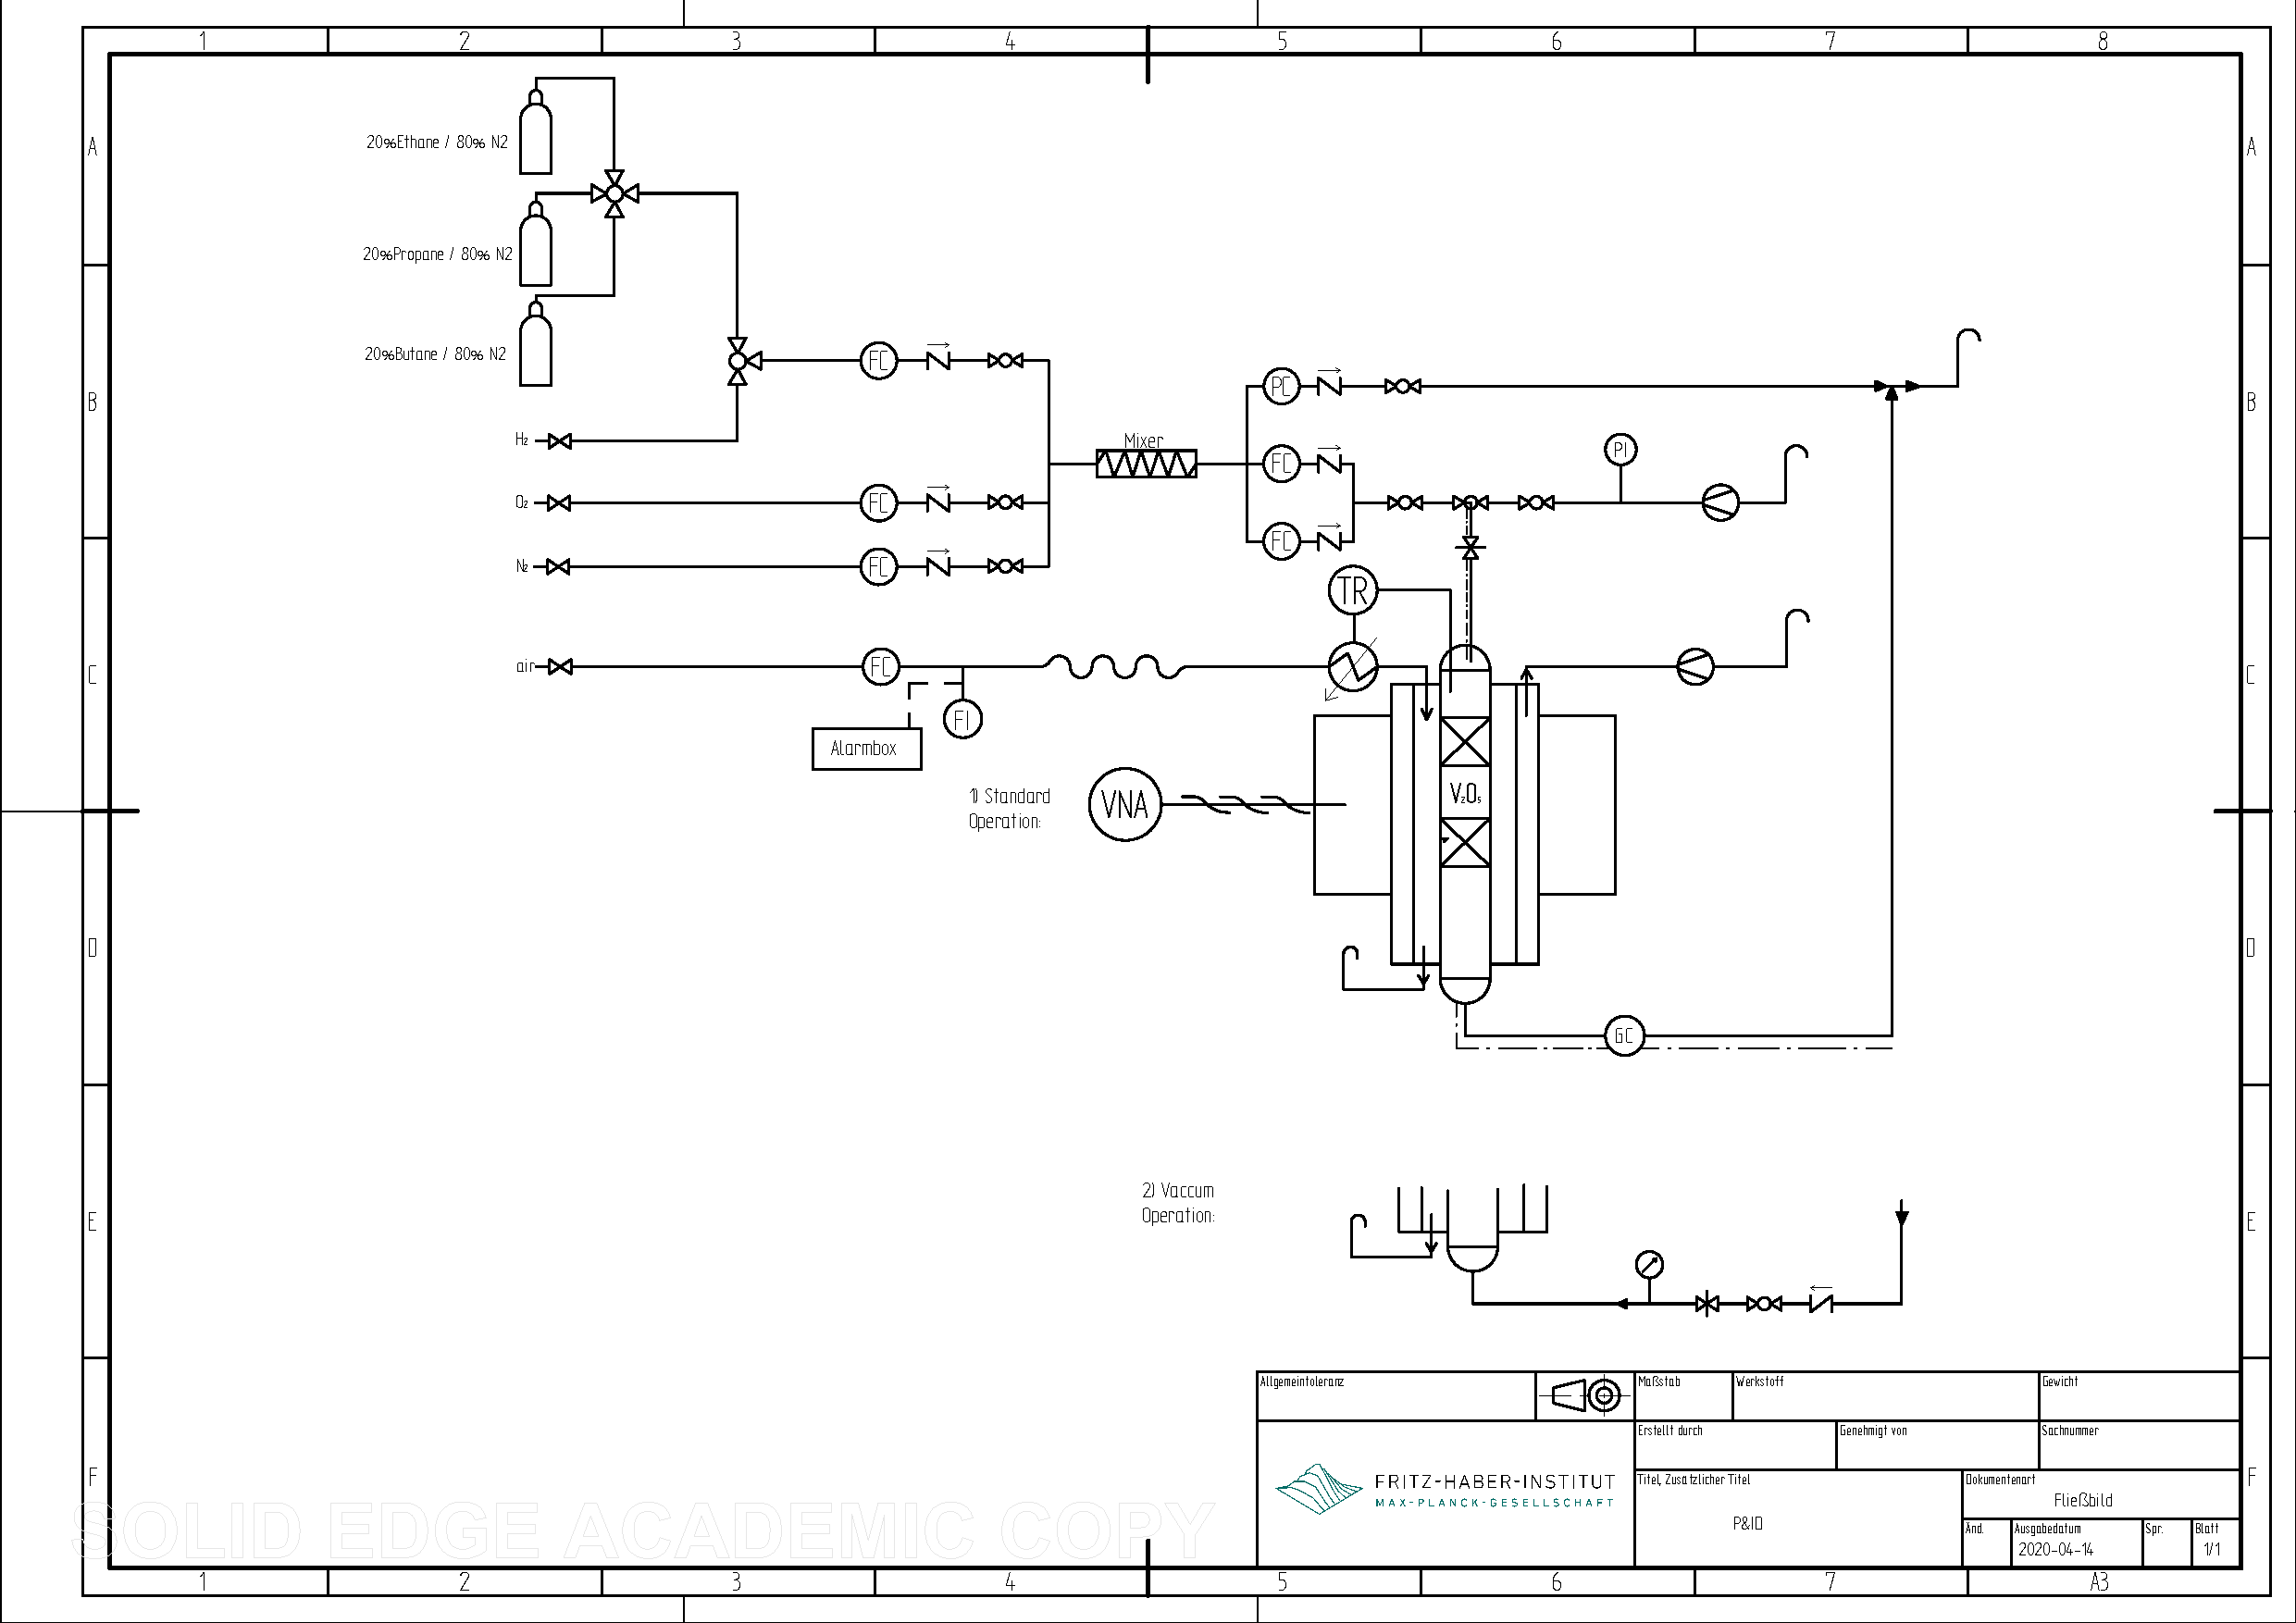
\includepdf[pages=1, landscape=True]{p+id_3.pdf}
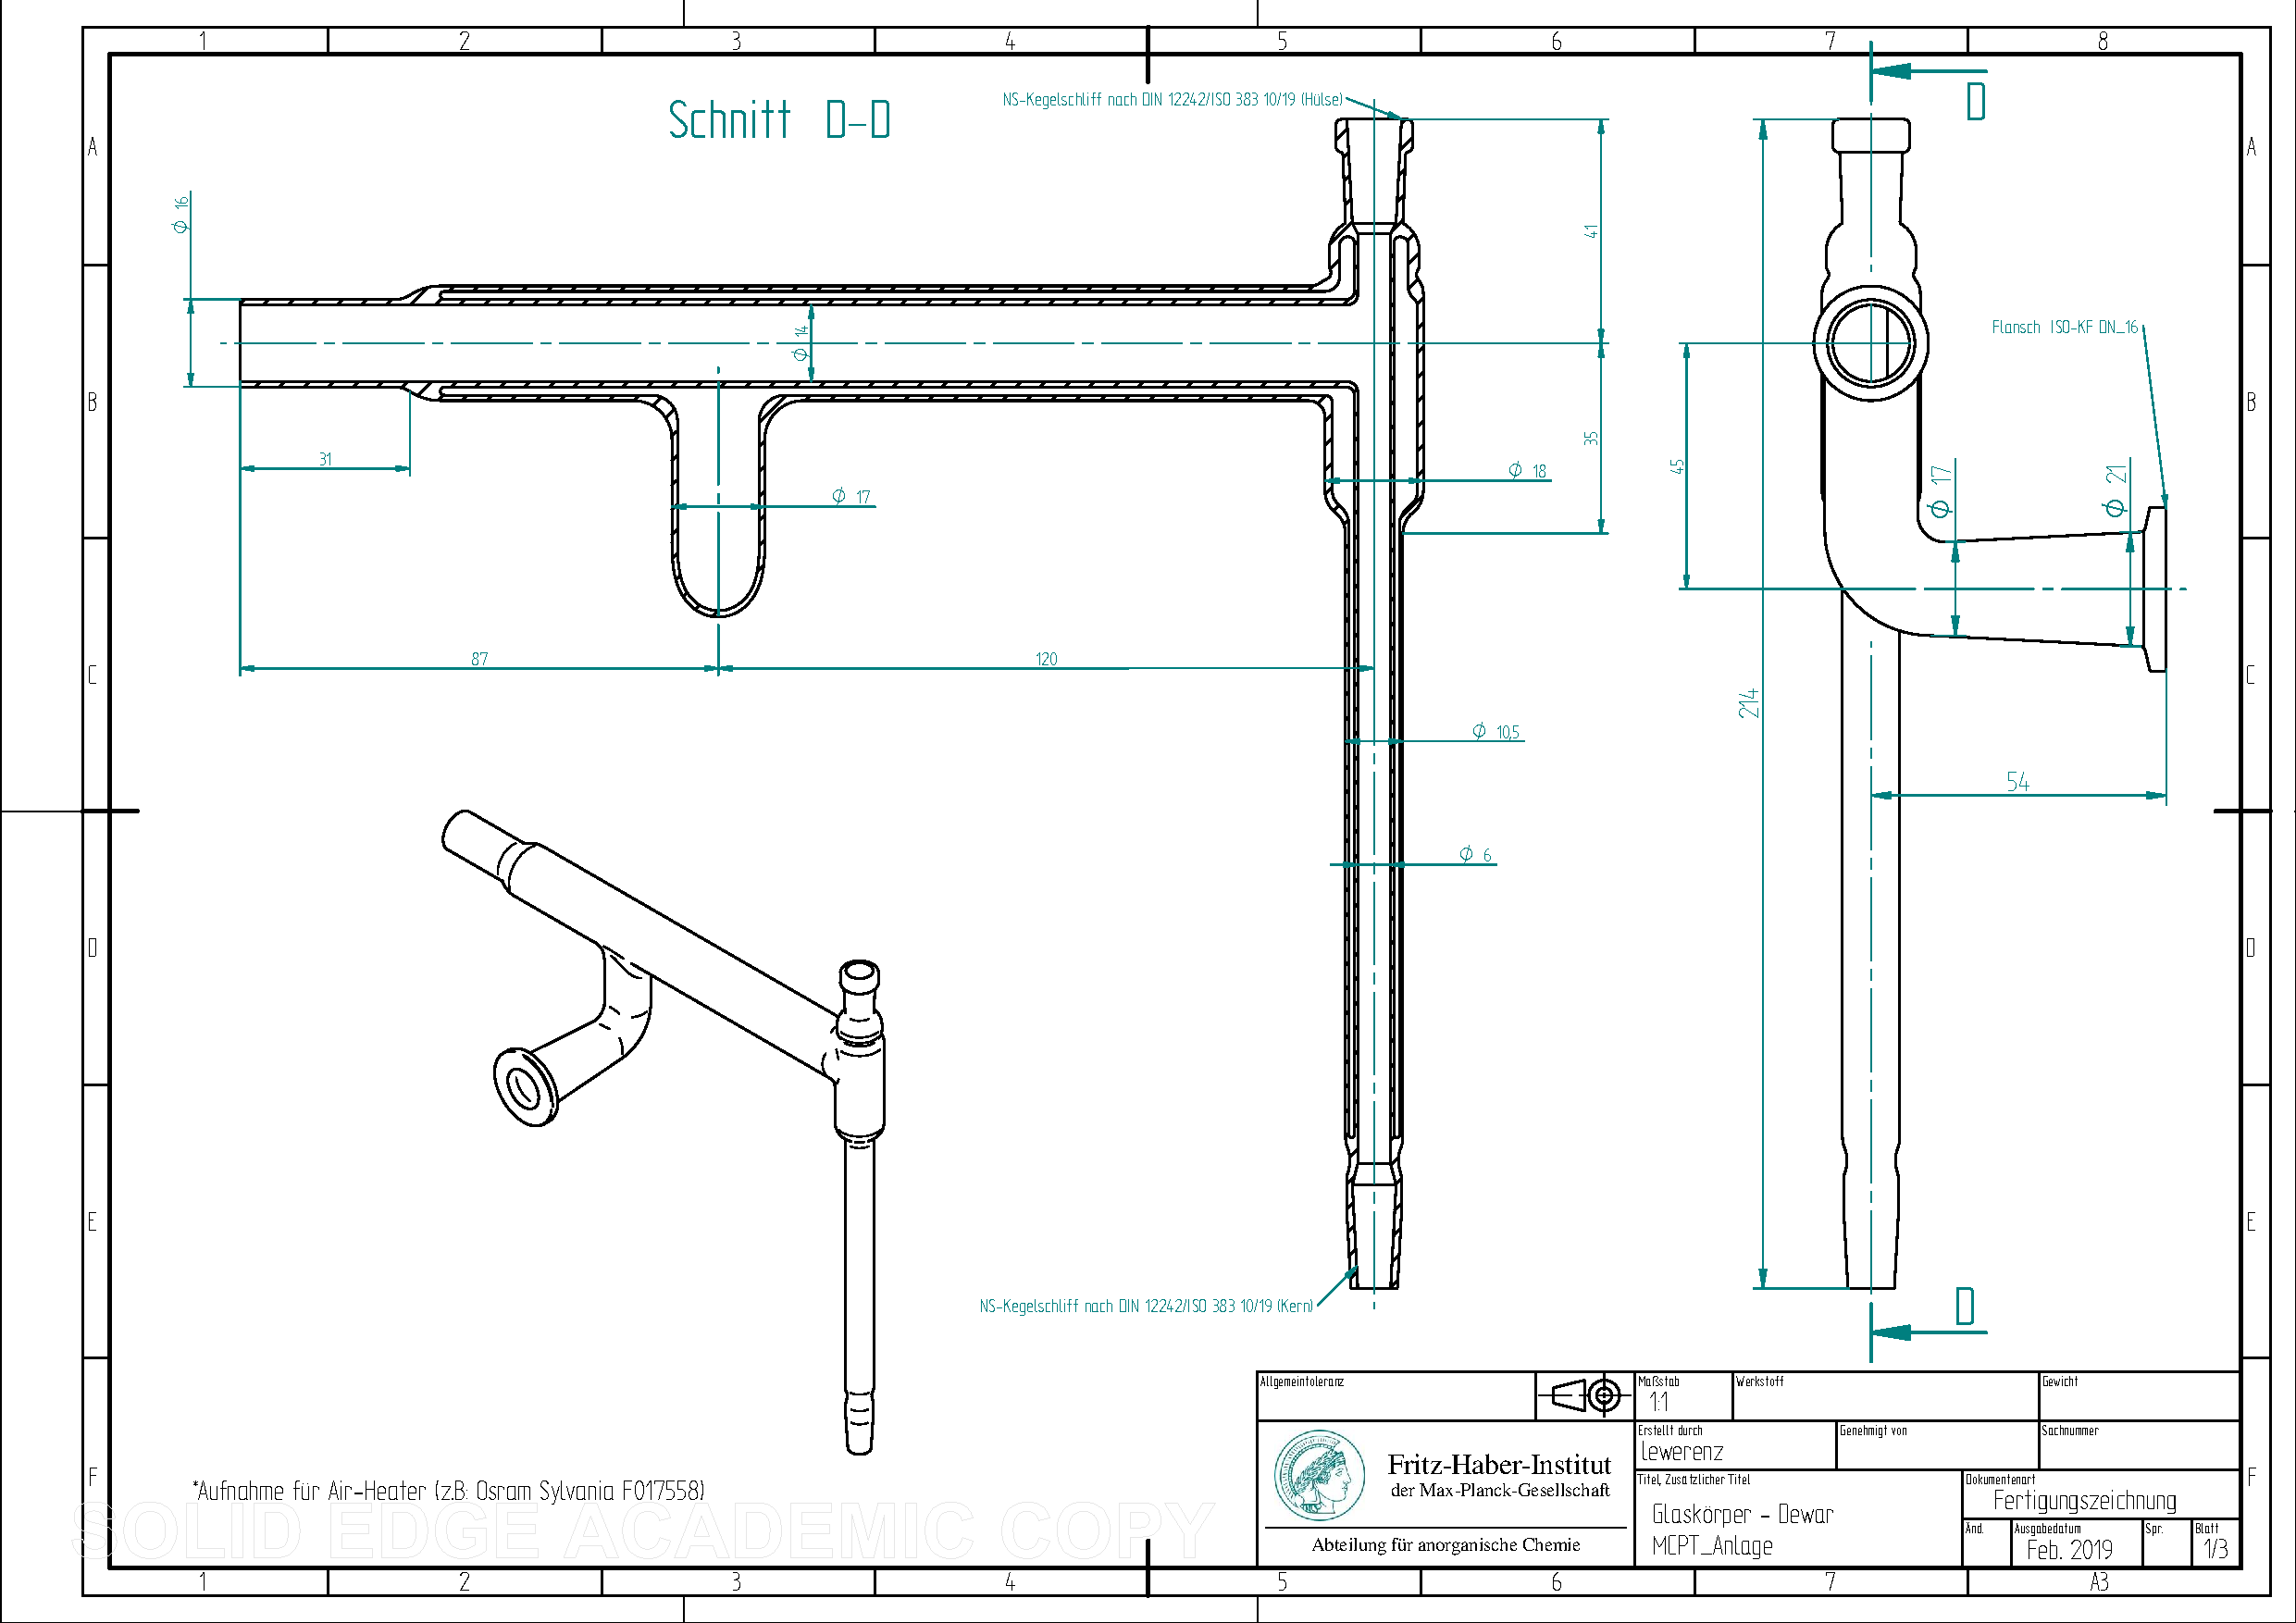
\includepdf[pages=1, landscape=True]{dewar.pdf}
\includepdf[pages=2, landscape=True]{dewar+reactor.pdf}
\includepdf[pages=3, landscape=True]{dewar+reactor.pdf}

\end{document}
